\subsubsection*{3a) Processes}
% chatpgt:
A \textbf{process} is a program in execution, an active entity with a program counter, registers, stack (temporary data), data section (global vars), and heap (dynamic mem). A program on disk is passive; it becomes a process when loaded into memory. The \textbf{Process Control Block (PCB)} stores context: state, registers, memory management, I/O status, scheduling, and accounting info. A \textbf{context switch} saves the state of an old process and loads the new one, introducing time overhead. Threads allow multiple sequences of execution within a process.

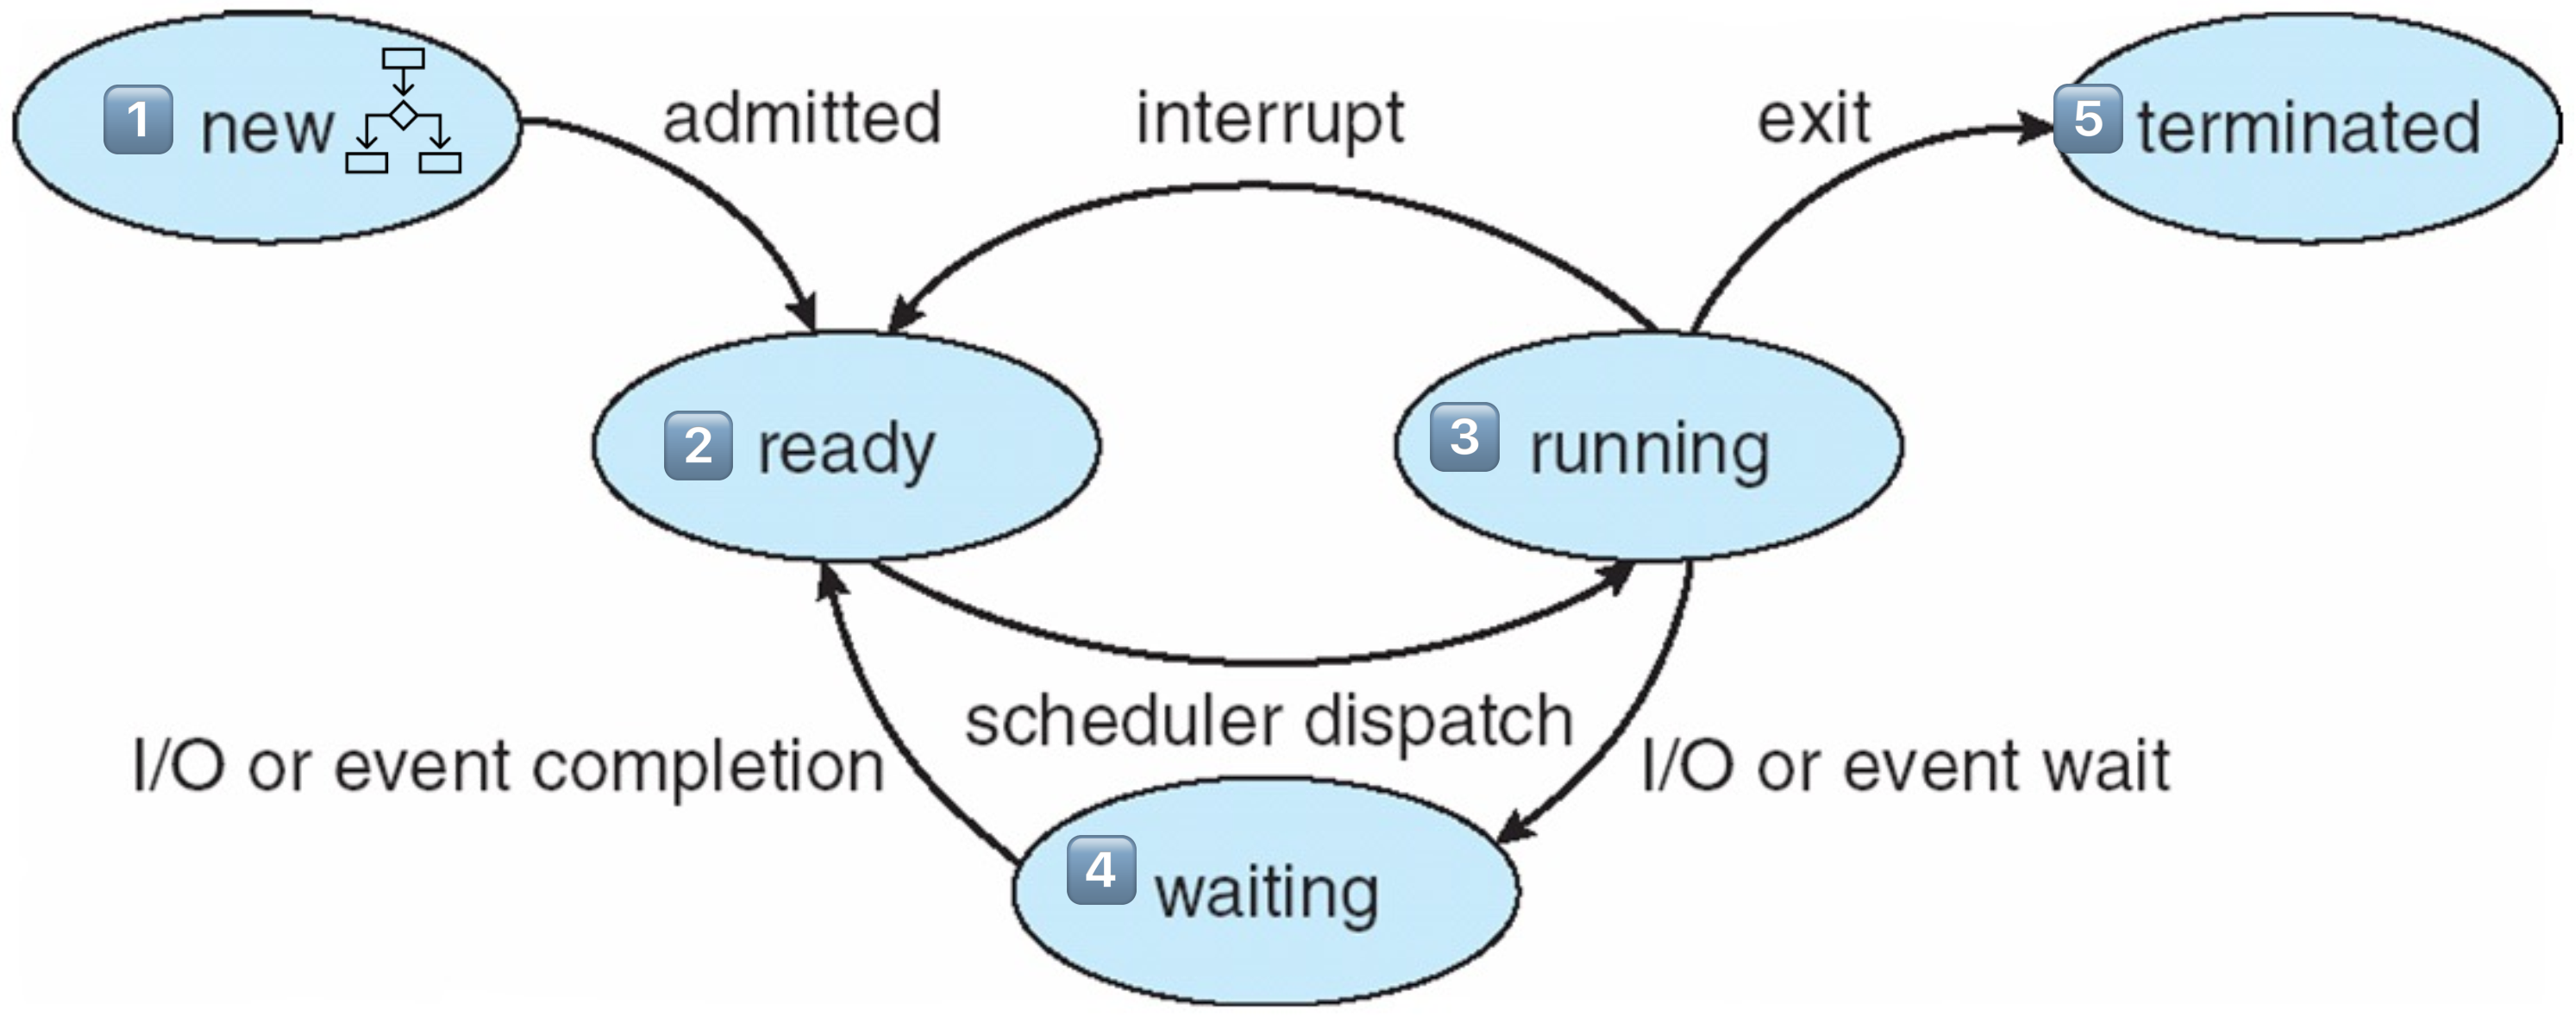
\includegraphics[width=0.95\linewidth]{images/03a_p09_process_states.png}

\textbf{Process scheduling} maximizes CPU utilization via multiprogramming/time-sharing. Processes are in the ready queue (waiting for CPU) or the wait queue (blocked on I/O or events). The \textbf{CPU scheduler} (short-term) selects processes for execution, while the \textbf{job scheduler} (long-term) controls degree of multiprogramming. The \textbf{medium-term scheduler} reduces load by suspending/resuming processes.

Processes can create other processes (forming a tree) with a unique PID. A child may inherit resources, execute concurrently or after the parent, share or copy address space. A process exits by \texttt{exit()} (parent may \texttt{wait()} for termination); a parent may \texttt{abort()} a child. Orphans are avoided by cascading termination. A \textbf{zombie} is a terminated child not yet \texttt{wait()}-ed for.

\textbf{Interprocess communication (IPC)} allows cooperating processes to share info. Two main models: \textbf{shared memory} (fast, but requires synchronization like producer-consumer patterns) and \textbf{message passing} (explicit send/receive, fixed or variable-sized messages, with links that can be direct or via mailboxes). IPC can be blocking (synchronous) or non-blocking (asynchronous); buffering can be zero, bounded, or unbounded. Examples: \textbf{pipes} (ordinary: parent-child only, named: general access) and \textbf{sockets} (for client-server comms, using TCP or UDP).


\subsubsection*{3b) Threads and Concurrency}

A \textbf{thread} is the smallest unit of CPU execution within a process. Threads share code, data, and OS resources but have independent program counters, registers, and stacks. Thread creation is lightweight compared to processes, enabling higher efficiency. Benefits include responsiveness, resource sharing, scalability, and simplified communication.

\textbf{Concurrency} (multiple tasks make progress) is interleaving execution of multiple tasks (sw). \textbf{Parallelism} is simultaneous execution of multiple tasks on multiple cores (hw). Modern CPUs have multiple cores, supporting both concurrency and parallelism. Work can be distributed by \textbf{data parallelism} (split data across threads) or \textbf{task parallelism} (split tasks).

\textbf{Amdahl's Law} estimates speedup from parallelization: $Speedup = 1 / (S + (1-S)/N)$, where $S$ is the serial portion.
Ignores parallelization overhead (e.g., task creation, contention, synchronization).
Serial portion limits speedup.

\textbf{(UT)}: managed in user space, invisible to kernel.
\textbf{(KT)}: managed and scheduled by kernel.

Thread models: \textbf{N:1} (many UT map to one KT), \textbf{1:1} (each UT has its own KT), and \textbf{M:N} (many UT multiplexed over KT). Some systems use a \textbf{Two-Level} model (hybrid of M:M with dedicated mappings).

% Thread model implications:
\textbf{N:1}: Blocking one user thread blocks all (only one kernel thread).
\textbf{1:1}: Higher concurrency, but thread count per process may be limited (kernel overhead).
\textbf{M:N}: Kernel can schedule another thread if one is blocked; avoids N:1 problem.
\textbf{Two-Level}: Some user threads have dedicated 1:1 mapping (e.g., for real-time or priority tasks).


Threads can be \textbf{explicit} (managed via API like Pthreads) or \textbf{implicit} (created by compilers/runtime). Thread \textbf{pools} pre-create threads for efficiency. \textbf{OpenMP} supports implicit parallelism via compiler directives in shared memory environments.

Thread issues: \textbf{fork/exec} behavior differs (fork duplicates, exec replaces). \textbf{Signals} notify processes of events (handled synchronously or asynchronously). \textbf{Thread cancellation} allows terminating threads, either asynchronously (immediate) or deferred (checked by the target thread).

\textbf{Thread-Local Storage (TLS)} gives threads private data accessible across function calls.
TLS is useful when you can't control thread creation (e.g., with implicit threading or thread pools).
\textbf{Provides data unique to each thread}, persistent across function calls (unlike local variables).


Process vs. Thread:
A \textbf{process} is a \textbf{container for resources} (e.g., memory, open files).
A \textbf{thread} is the \textbf{execution entity} with instructions and context.
Even in a single-threaded process, it's the \textbf{thread that is scheduled} by the OS.

\textbf{T vs P usage: }Threads for tasks needing \textbf{frequent communication and shared state}.
Processes for \textbf{higher separation \& security}.

Linux treats threads as processes (no strict distinction); \texttt{clone()} creates threads, \texttt{fork()} creates separate processes. Threads share resources if specified by \texttt{clone()} flags.

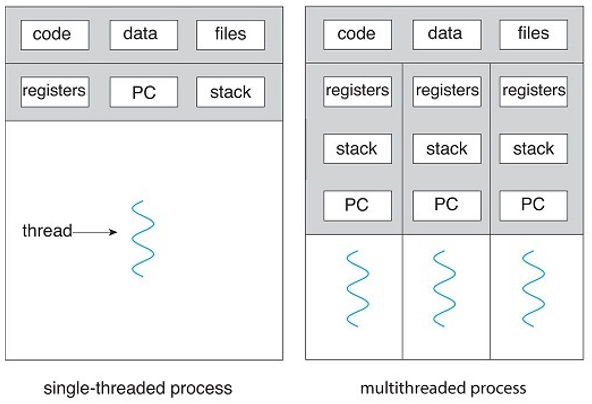
\includegraphics[width=0.95\linewidth]{images/03a_p14_threaded_process.png}

\subsubsection*{3c) CPU Scheduling}

A process alternates between CPU and I/O bursts. CPU-bound processes have few long bursts; I/O-bound processes have many short bursts. Scheduling selects which process/thread to execute: \textbf{short-term scheduler} chooses from the ready queue, \textbf{long-term scheduler} controls the degree of multiprogramming, \textbf{medium-term scheduler} may swap processes out.

\textbf{Preemptive} scheduling interrupts running processes (risk of race conditions, must handle in kernel mode). \textbf{Non-preemptive} scheduling waits for process to release CPU voluntarily. The \textbf{dispatcher} handles context switching, moving from the old to the new process, introducing latency (ideally <$10\mu$s).

\textbf{Scheduling criteria}: maximize CPU utilization, throughput (completed processes/time), minimize turnaround time (completion time - arrival), waiting time (in ready queue), response time (submission to first response).

\textbf{Algorithms}:
\textbf{FCFS} (non-preemptive): simple but poor response for short processes (convoy effect).
\textbf{SJF}: optimal (minimum average waiting), predicts next burst via exponential averaging.
\textbf{Priority}: fixed or dynamic, risk of starvation; \textbf{aging} prevents starvation by increasing priority over time.  
\textbf{RR} (round robin): time-sliced FCFS, preempts after quantum; quantum too small → overhead, too large → FCFS-like behavior.  
\textbf{MLQ} (multilevel queue): queues per priority/type, fixed scheduling per queue (e.g., RR for foreground, FCFS for background), may starve lower-priority queues.
\textbf{MLFQ}: feedback mechanism allows movement between queues; short bursts → high priority, long bursts → demoted. Most flexible but complex.
\textbf{CFS} (Completely Fair Scheduler, Linux): proportional fair share; tasks with lower \texttt{vruntime} get CPU, stored in a red-black tree (O(log n)); preemptive, priority via \texttt{nice} value. Real-time tasks (0-99) have static priority, normal tasks (100-139) get dynamic fair share.

\textbf{Thread scheduling}: threads (user or kernel-level) compete within the process (\textbf{PCS}) or system-wide (\textbf{SCS}); kernel threads scheduled by OS (one-to-one model), user threads by library (many-to-one/many-to-many).  

\textbf{Multiprocessor scheduling}: cores can share queues or have per-core queues (better affinity). Load balancing via \textbf{push} (force move) or \textbf{pull} (steal work). \textbf{Processor affinity}: keeps threads on the same core for cache locality (soft/hard affinity). \textbf{NUMA-aware scheduling} places threads near memory for lower latency. \textbf{Heterogeneous multicore systems} (e.g., big.LITTLE) mix cores of different performance/power profiles.

\textbf{Algorithm evaluation}: deterministic (static workloads), queueing models (Little's Law: $N=\lambda W$), simulations, or real system tests.